\section{Ход работы}
\subsection{Измерения}

1. Некоторые данныеиз справочных материалов:
\[2r_1 = 50 \pm 3 \text{ мкм, -- диаметр нити;}\]
\[2r_0 = 7,0 \pm 0,1 \text{ мм, -- диаметр колбы;}\]
\[\ln \frac{r_0}{r_1} = 5\]
\[L = 400 \pm 2 \text{ мм, -- длина нити;}\]
\[R_\text{н} \sim  20 \text{ Ом, -- сопротивление нити;}\]
\[\varepsilon_\text{уст} = 3,2 \text{ В, -- напряжение на источнике питания.}\]

2. В целях безопасности посчитаны максимальные мощность, сила тока и напряжение для нити:
\[Q_{max} = 3770 \text{ мВт},\]
\[U_{max} = 8,7 \text{ В},\]
\[I_{max} = 433 \text{ мА}.\]

3. Для разных температур измерены напряжение и сила тока на нити представлены в таблицах 1-4
\begin{table}
    \begin{tabular}{|c|c|c|c|}
    \hline
    I, мА & U, В & Q, мВт & R, Ом \\
    \hline
    15.4 & 0.314 & 4.836 & 20.39 \\
    \hline
    43.87 & 0.901 & 39.527 & 20.538 \\
    \hline
    57.81 & 1.195 & 69.083 & 20.671 \\
    \hline
    67.74 & 1.412 & 95.649 & 20.844 \\
    \hline
    75.27 & 1.579 & 118.851 & 20.978 \\
    \hline
    81.45 & 1.716 & 139.768 & 21.068 \\
    \hline
    86.77 & 1.838 & 159.483 & 21.182 \\
    \hline
    91.36 & 1.945 & 177.695 & 21.289 \\
    \hline
    95.2 & 2.032 & 193.446 & 21.345 \\
    \hline
    98.98 & 2.122 & 210.036 & 21.439 \\
    \hline
    102.31 & 2.201 & 225.184 & 21.513 \\
    \hline
    \end{tabular}
\hfill
    \begin{tabular}{|c|c|c|c|}
    \hline
    I, мА & U, В & Q, мВт & R, Ом \\
    \hline
    15.23 & 0.323 & 4.919 & 21.208 \\
    \hline
    42.99 & 0.919 & 13.996 & 21.377 \\
    \hline
    56.56 & 1.217 & 18.535 & 21.517 \\
    \hline
    66.45 & 1.44 & 21.931 & 21.67 \\
    \hline
    73.82 & 1.609 & 24.505 & 21.796 \\
    \hline
    79.69 & 1.745 & 26.576 & 21.897 \\
    \hline
    84.85 & 1.867 & 28.434 & 22.004 \\
    \hline
    89.15 & 1.969 & 29.988 & 22.086 \\
    \hline
    93.03 & 2.061 & 31.389 & 22.154 \\
    \hline
    96.38 & 2.144 & 32.653 & 22.245 \\
    \hline
    99.71 & 2.224 & 33.872 & 22.305 \\
    \hline
    \end{tabular}
\hfill
    \begin{tabular}{|c|c|c|c|}
    \hline
    I, мА & U, В & Q, мВт & R, Ом \\
    \hline
    15.2 & 0.333 & 5.062 & 21.908 \\
    \hline
    42.61 & 0.941 & 40.096 & 22.084 \\
    \hline
    55.89 & 1.243 & 69.471 & 22.24 \\
    \hline
    65.55 & 1.466 & 96.096 & 22.365 \\
    \hline
    72.75 & 1.636 & 119.019 & 22.488 \\
    \hline
    78.5 & 1.773 & 139.181 & 22.586 \\
    \hline
    83.48 & 1.893 & 158.028 & 22.676 \\
    \hline
    87.66 & 1.995 & 174.882 & 22.758 \\
    \hline
    91.2 & 2.083 & 189.97 & 22.84 \\
    \hline
    94.6 & 2.161 & 204.431 & 22.844 \\
    \hline
    97.71 & 2.246 & 219.457 & 22.986 \\
    \hline
    \end{tabular}
\hfill
\begin{tabular}{|c|c|c|c|}
    \hline
    I, мА & U, В & Q, мВт & R, Ом \\
    \hline
    15.12 & 0.342 & 5.17104 & 22.619 \\
    \hline
    42.21 & 0.962 & 40.606 & 22.7908 \\
    \hline
    55.21 & 1.266 & 69.8959 & 22.9306 \\
    \hline
    64.63 & 1.491 & 96.3633 & 23.0698 \\
    \hline
    71.65 & 1.66 & 118.939 & 23.1682 \\
    \hline
    77.19 & 1.796 & 138.633 & 23.2673 \\
    \hline
    81.96 & 1.914 & 156.871 & 23.3529 \\
    \hline
    85.98 & 2.015 & 173.25 & 23.4357 \\
    \hline
    89.41 & 2.101 & 187.85 & 23.4985 \\
    \hline
    92.67 & 2.185 & 202.484 & 23.5783 \\
    \hline
    95.67 & 2.262 & 216.406 & 23.6438 \\
    \hline
\end{tabular}
\hfill
    \begin{tabular}{|c|c|c|c|}
    \hline
    I, мА & U, В & Q, мВт & R, Ом \\
    \hline
    15.07 & 0.352 & 5.30464 & 23.3577 \\
    \hline
    41.78 & 0.982 & 41.028 & 23.5041 \\
    \hline
    54.51 & 1.288 & 70.2089 & 23.6287 \\
    \hline
    63.68 & 1.513 & 96.3478 & 23.7594 \\
    \hline
    70.45 & 1.681 & 118.426 & 23.8609 \\
    \hline
    75.87 & 1.817 & 137.856 & 23.9489 \\
    \hline
    80.54 & 1.936 & 155.925 & 24.0377 \\
    \hline
    84.45 & 2.037 & 172.025 & 24.1208 \\
    \hline
    87.83 & 2.125 & 186.639 & 24.1945 \\
    \hline
    91.01 & 2.206 & 200.768 & 24.2391 \\
    \hline
    93.71 & 2.278 & 213.471 & 24.309 \\
    \hline
    \end{tabular}
\end{table}
\subsection{Обработка}

4. По таблицам строим графики $R(Q)$.
\begin{figure}[h]
    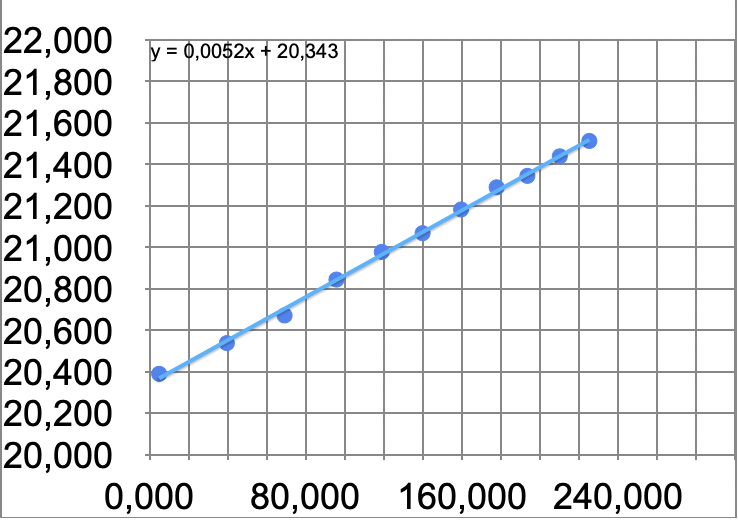
\includegraphics[width = 0.7\linewidth]{23.png}
    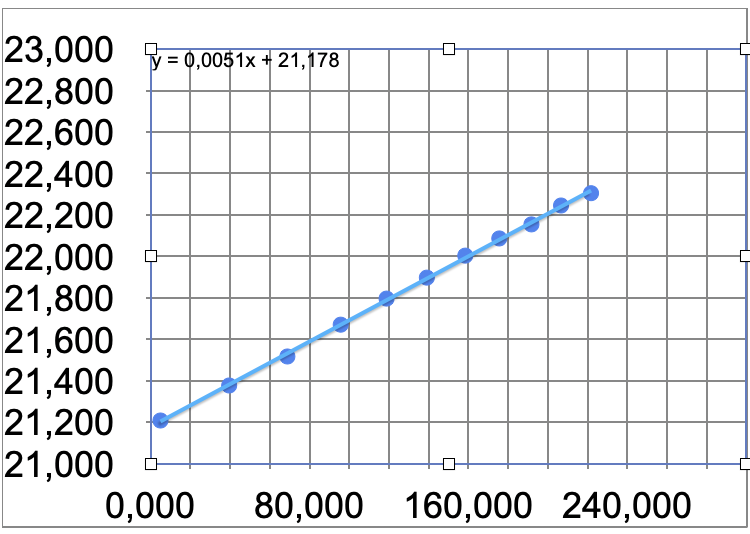
\includegraphics[width = 0.7\linewidth]{35.png}
\end{figure}
\begin{figure}[h]
    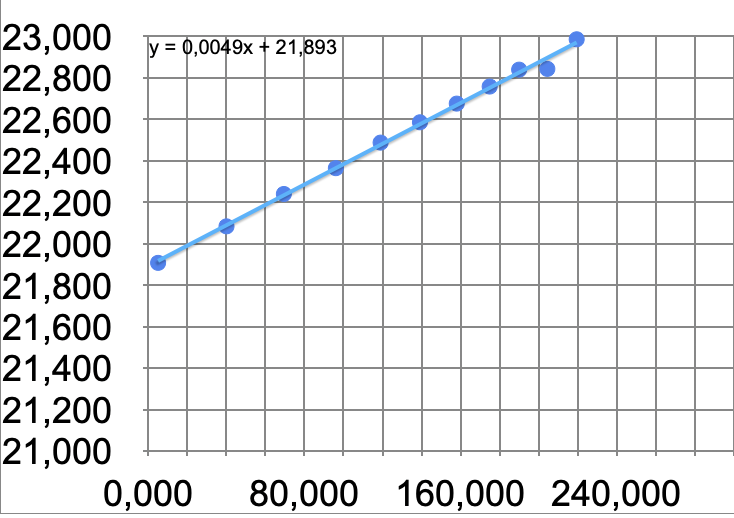
\includegraphics[width = 0.7\linewidth]{45.png}
    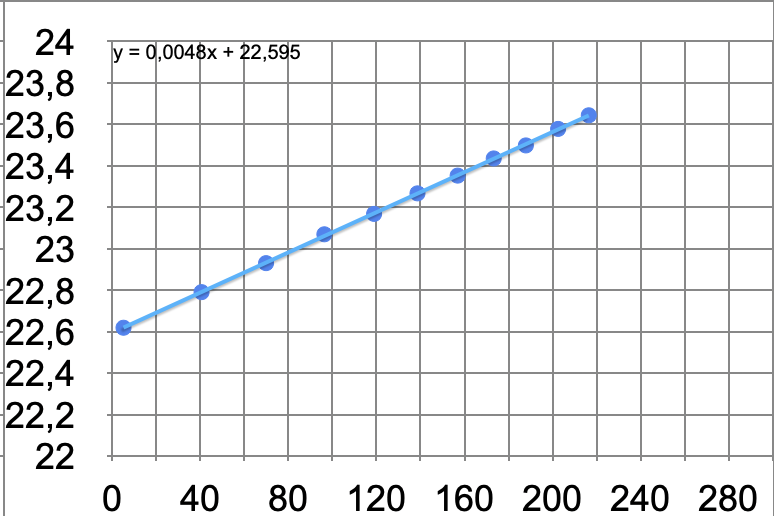
\includegraphics[width = 0.7\linewidth]{55.png}
    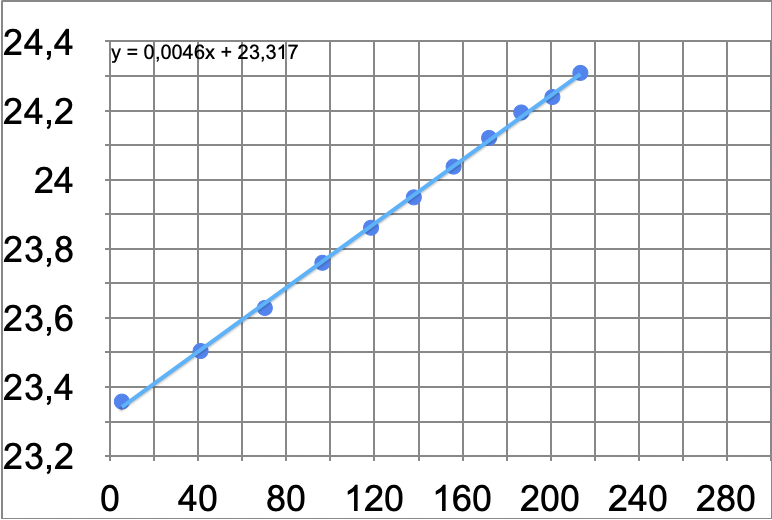
\includegraphics[width = 0.7\linewidth]{65.png}
\end{figure}

5. По грфикам определим $R_0$ для каждой температуры:
\[R_{0\left(T = 23^\circ C\right)} = 20.3 \pm 0.5 \text{ Ом},\]
\[R_{0\left(T = 35^\circ C\right)} = 21.2 \pm 0.5 \text{ Ом},\]
\[R_{0\left(T = 45^\circ C\right)} = 21.9 \pm 0.6 \text{ Ом},\]
\[R_{0\left(T = 55^\circ C\right)} = 22.6 \pm 0.8 \text{ Ом},\]
\[R_{0\left(T = 65^\circ C\right)} = 23.3 \pm 0.6 \text{ Ом},\]

6. Зависимость $R_0 (T)$
\begin{figure}[h]
    \includegraphics*{R_0(T).png}
    % \caption{$R_0(T)$}
\end{figure}

Получились результаты: $\frac{dR_0}{dT} = 0.071 \pm 0.004 \text{ }\frac{\text{Ом}}{\text{K}}$, $\alpha = \frac{1}{R_{273}}\frac{dR_0}{dT} = (3.8 \pm 0.3) \cdot 10^{-3} \text{ K}^{-1}$

7. Получим зависимость $\frac{dQ}{d(\Delta T)} = \frac{dR}{dT} / \frac{dR}{dQ}$ для каждого случая
\begin{table}[h]
\centering
\begin{tabular}{|c|c|c|}
    \hline
    T, $^\circ C$ & $\frac{dQ}{d(\Delta T)}$, $10^{-2} \text{ } \frac{\text{Вт}}{K} $ & $\kappa$, $10^{-3}\text{ }\frac{\text{Вт}}{K \cdot \text{м}}$\\
    \hline
    23 & 1.36 & 27.1 \\
    \hline
    35 & 1.39 & 27.7 \\
    \hline
    45 & 1.44 & 28.6 \\
    \hline
    55 & 1.48 & 29.4 \\
    \hline
    65 & 1.54 & 30.6 \\
    \hline
\end{tabular}
\end{table}

8. Построим график $\ln\kappa(\ln T)$.
\begin{figure}[h]
    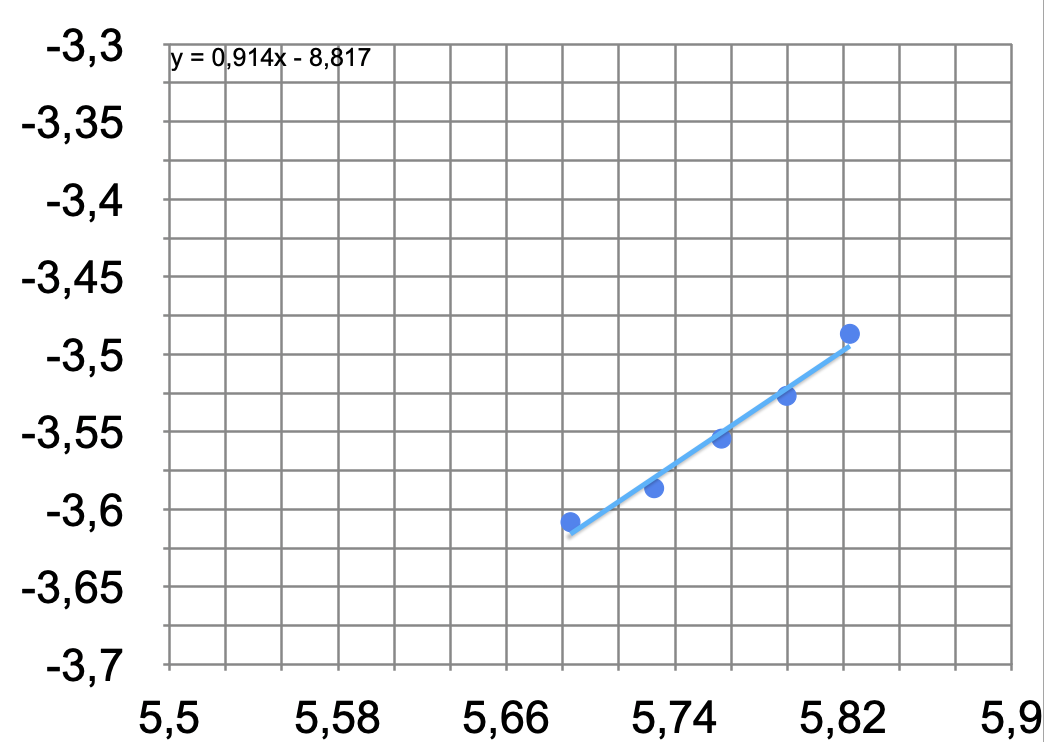
\includegraphics[width = \linewidth]{lnk.png}
\end{figure}
Получилось $\beta = 0.9 \pm 0.3$.
